\subsection*{Database Design}
\addcontentsline{toc}{subsection}{Database Design}
	For the database of CAMEL, we have decided to to take the pre-existing database and modify it to suit the needs of the new intended parser. Much of the models that were already provided will be used, though there will be some changes with them, such as BookNode and TextNode. The possible limitation of changing the current models will mean that current code may not be compatible. However as we intent to re-write much of the current code this should not be an issue. One design aspect that we have already applied to CAMEL was separating each model to now reside in its appropriate application rather than being in one cluttered file. This can be seen in the code that is attached.\\ 
	
	The models that will be included in CAMEL:
	\begin{itemize}
		\item \textbf{BookNode}: This object relates to different Latex components that make up the whole document. Each BookNode contains a parent node, unless it is the root node, which remains null. Each node has a parent as this allows Django - MPTT to traverse through the nodes to generate a page. The BookNode is used in other models, such as 'Submission' and 'Module' to provide links to relevant pages.     
		
		\item \textbf{TextNode}: Each TextNode contains the any text that was contained inside latex markup. These objects will contain the relevant information that will be outputted by Django - MPTT when it renders the relevant HTML during the web page rendering process. Each TextNode has a parent BookNode, which contains the location for it.  
		
		\item \textbf{Book}: Book is the object that will provide a connection between the BookNode object and the Module object. This allows modules to select which books are relevant and add them to the list that the student can access. The Book object will take a 'root' (start of latex book) BookNode object to allow this connection. 
		
		\item \textbf{Module}: This model relates to the module a student will take. It will contain the current year of study and provides a link for students to access relevant books as well as tasks that are required to be completed. Each module will contain a number of relevant books for them to study from.
		
		\item \textbf{Submission}: The submission object will be used to submit all answers that a student has entered from objects 'SingleChoiceAnswer' and 'Answer.' With each of these submissions, it will not allow a lecturer to access any of their details, such as their name. This allows the submissions to keep with university policy concerning anonymous marking. A student can only submit a quiz or homework once from each task in a book.   
		
		\item \textbf{SingleChoiceAnswer}: This object is used to hold the answers from the multiple choice questions that are on CAMEL. This object allows the student to save and comeback later to the question. The answer is stored in the object and is used with 'Submission' to allow a student to submit their answers. 
		
		\item \textbf{Answer}: Answer is the object that is used to store the answer from a question from the UI input box. This will hold any latex that the student enters and can be viewed on the question on the UI side. This also will be used to save the answer for submission. Like 'SingleChoiceAnswer,' the answer entered can be saved and continued later on. 
	\end{itemize}
	
	We will also be utilising some pre-existing tables that have been included with Django. One of these is Users which is the backbone of creating the Students, Administrator and Lecturer accounts. We have decided to use this table as it provides much of the functionality that we need in terms of security that could take some time to implement ourselves. For example, restrictions can be easily applied as Django has already provided this functionality. Additionally, security is greater with using User as Django has also provided a 'hash and salt' hashing mechanism in the table to protect user passwords.\\	
	
	\begin{figure}[h]
		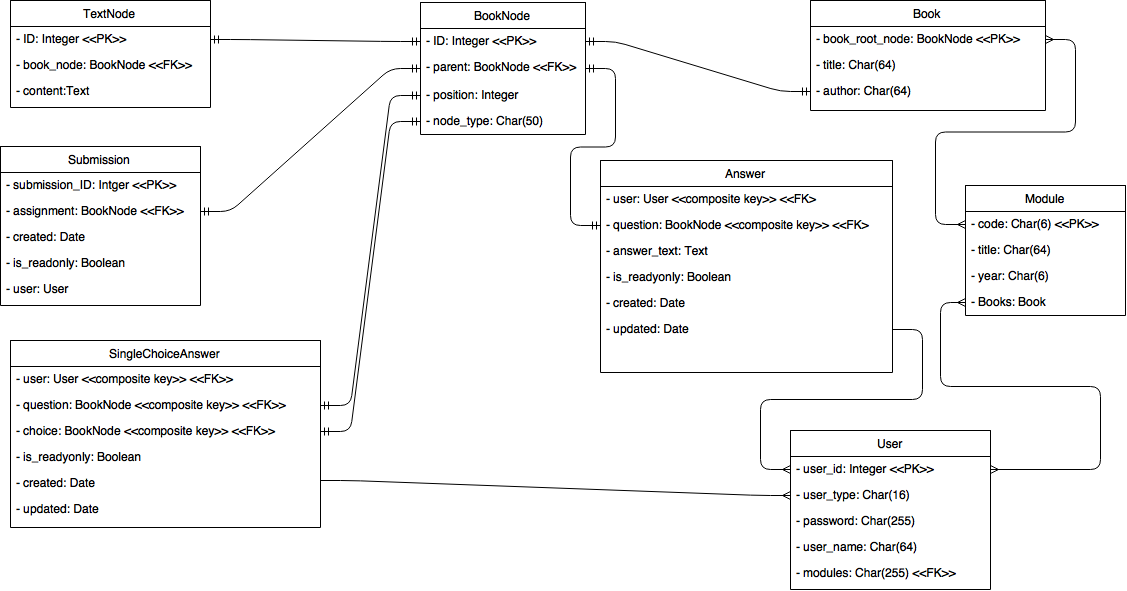
\includegraphics[scale=0.45]{img/database_design}
		\caption{CAMEL Database Design}
	\end{figure}
	
	Above is the database design with all the models that will be implemented into the final CAMEL system. As you can see from the diagram, BookNode is one of the main models that CAMEL is reliant on. The advantage of the MVC architecture is that these modules are separate from any other code that interacts with them, so any changes that are made for design reasons can be successfully implemented. The possible limitation that could occur with the design above is bottlenecks with many requests for the BookNode objects, when placed live with students. Extensive testing will be needed here to see if there are performance issues with this.\\